\documentclass{article}
\usepackage[utf8]{inputenc}
\usepackage{graphicx}
\usepackage{listings}
\usepackage[dvipsnames]{xcolor}
\usepackage{amsmath}
\usepackage{hyperref}

\newcommand{\sectionlinetwo}[2]{%
  \nointerlineskip \vspace{.5\baselineskip}\hspace{\fill}
  {\color{#1}
    \resizebox{0.5\linewidth}{2ex}
    {{%
    {\begin{tikzpicture}
    \node  (C) at (0,0) {};
    \node (D) at (9,0) {};
    \path (C) to [ornament=#2] (D);
    \end{tikzpicture}}}}}%
    \hspace{\fill}
    \par\nointerlineskip \vspace{.5\baselineskip}
  }
\definecolor{azure}{rgb}{0.0, 0.5, 1.0}
\definecolor{forestgreen}{rgb}{0.13, 0.55, 0.13}
\definecolor{codegreen}{rgb}{0,0.6,0}
\definecolor{codegray}{rgb}{0.5,0.5,0.5}
\definecolor{codepurple}{rgb}{0.58,0,0.82}
\definecolor{backcolour}{rgb}{0.95,0.95,0.92}

\lstdefinestyle{mystyle}{
    backgroundcolor=\color{backcolour},   
    commentstyle=\color{codegreen},
    keywordstyle=\color{magenta},
    numberstyle=\tiny\color{codegray},
    stringstyle=\color{codepurple},
    basicstyle=\ttfamily\footnotesize,
    breakatwhitespace=false,         
    breaklines=true,                 
    captionpos=b,                    
    keepspaces=true,                 
    numbers=left,                    
    numbersep=5pt,                  
    showspaces=false,                
    showstringspaces=false,
    showtabs=false,                  
    tabsize=2
}
\lstset{style=mystyle}

\title{Submission for HW 1\\\small{\textit{CS 427: Mathematics for Data Science, Autumn 2020-21}}}
\author{K. Sai Anuroop, 170030035}
\date{\today}

\begin{document}

\maketitle

\begin{flushleft}
\textbf{Solution 1}\\~\\
Let $x_{1},x_{2}\in C$ defined by $C=\{x\mid Ax=b\}$, where $A\in R^{m\times n}$, $b\in R^{m}$ and $\theta\in R$. Then\\
$A(\theta x_{1}+(1-\theta)x_{2})=\theta Ax_{1}+(1-\theta)Ax_{2}=\theta b+(1-\theta)b=b$
$\Rightarrow \theta x_{1}+(1-\theta)x_{2}\in C$\\
So, $C$ \textbf{is} an affine set.\\~\\

\textbf{Solution 2}
\begin{enumerate}
	\item $\textbf{aff}\ C=\{x \in R^{3}\mid x_{3}=0\}$
	\item $\textbf{conv}\ C=C$
	\item $\textbf{int}\ C=\phi$
	\item $\textbf{relint}\ C=\{x\in R^{3}\mid-1<x_{1}<1,-1<x_{2}<1,x_{3}=0\}$
\end{enumerate}
\textbf{Solution 3}\\~\\
% TODO
Let $P=
\Bigg(\begin{matrix}
  1 & 0\\
  0 & -1
\end{matrix}\Bigg) \in R^{2 \times 2}$ and $c=\Bigg(\begin{matrix}
  0.5\\
  0.5
\end{matrix}\Bigg)$, $x_{1}=\Bigg(\begin{matrix}
  1\\
  1
\end{matrix}\Bigg)$, $x_{2}=\Bigg(\begin{matrix}
  1\\
  -1
\end{matrix}\Bigg) \in R^{2}$\\
Note that $c^{T}x_{1}=1$ and $c^{T}x_{2}=0$, $x_{1}^{T}Px_{1}=0$ and $x_{2}^{T}Px_{2}=0$. So, $x_{1}, x_{2} \in C$ where $C=\{x\mid x^{T}Px\leq (c^{T}x)^{2}, c^{T}x\geq 0\} \ \forall\  c,x \in R^{2}, P\in R^{2\times 2}$\\
Let $0\leq\theta\leq1$. Consider $\theta x_{1}+(1-\theta x_{2})=\Bigg(\begin{matrix}
  1\\
  2\theta-1
\end{matrix}\Bigg)$\\
Note that $c^{T}(\theta x_{1}+(1-\theta)x_{2})=\theta \in [0,1]$\\
Also note that $(\theta x_{1}+(1-\theta)x_{2}))^{T}P(\theta x_{1}+(1-\theta)x_{2})=4\theta-4\theta^{2}$.\\
However, for $\theta\in\Big(0,\dfrac{4}{5}\Big)$, $4\theta-4\theta^{2}>\theta^{2}$\\
This means $(\theta x_{1}+(1-\theta)x_{2})^{T}P(\theta x_{1}+(1-\theta)x_{2})>(c^{T}(\theta x_{1}+(1-\theta)x_{2}))^{2}\ \forall\  \theta \in \Big(0,\dfrac{4}{5}\Big)$.\\
$\Rightarrow (\theta x_{1}+(1-\theta)x_{2})\not \in C\  \forall\  \theta \in \Big(0,\dfrac{4}{5}\Big)$.\\
So, $C$ is \textbf{not} convex.
\clearpage
\textbf{Solution 4}
\begin{enumerate}
	\item Plot of $f(x)=x^{2}\   \forall x \in[-10,10]$
	\begin{figure}[htp]
		\centering
		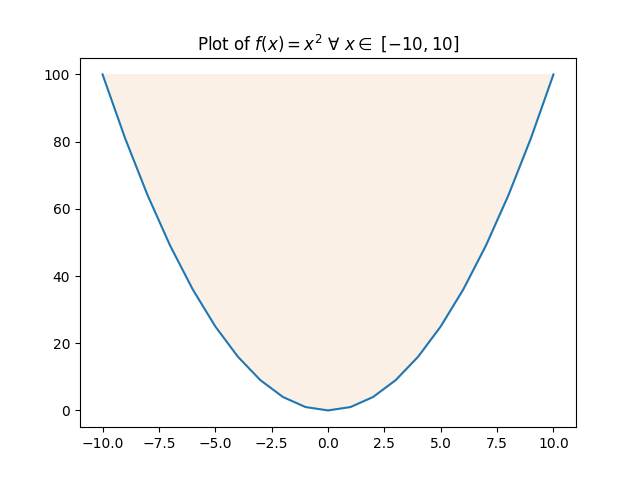
\includegraphics[width=9cm]{x2.png}
	\end{figure}
	\item Plot of $f(x)=\sin(x)\   \forall x \in[-2\pi,2\pi]$
	\begin{figure}[htp]
		\centering
		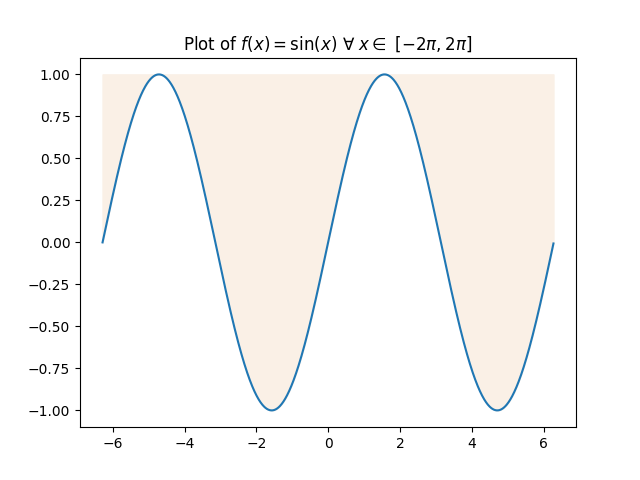
\includegraphics[width=9cm]{sinx.png}
	\end{figure}
	\clearpage
	\item Plot of $f(x,y)=(xy)^{2}\   \forall x,y \in[-10,10]$
	\begin{figure}[htp]
		\centering
		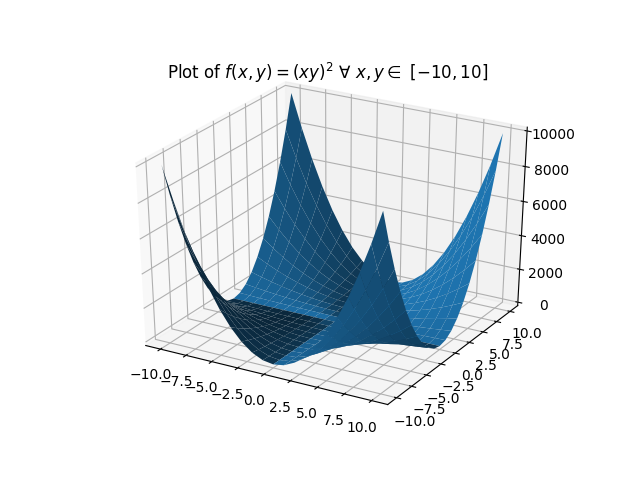
\includegraphics[width=9cm]{xy2.png}
	\end{figure}
	\item Contour plot of $f(x,y)=(xy)^{2}\   \forall x,y \in[-10,10]$
	\begin{figure}[htp]
		\centering
		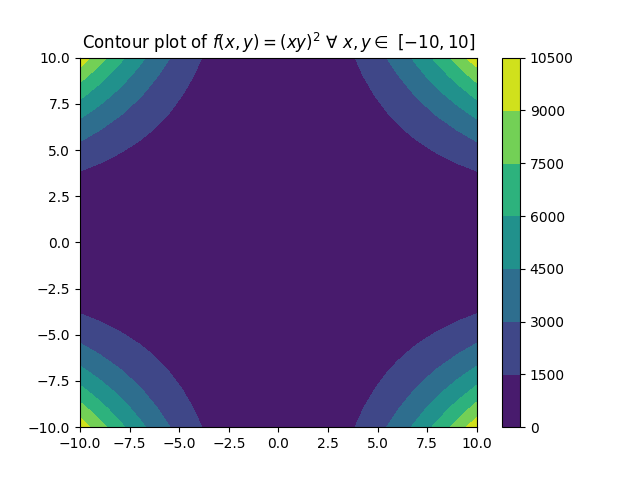
\includegraphics[width=9cm]{xy2contour.png}
	\end{figure}
\end{enumerate}
\clearpage
\begin{lstlisting}[language=Python, title={Python code to generate the plots in \textbf{Solution 4}}]
import numpy as np  
import matplotlib.pyplot as plt  
from mpl_toolkits import mplot3d

def x2():
    x0 = np.array(range(-10, 11))
    y0 = eval('x0**2')
    plt.fill_between(x0, y0, 100, color='linen')
    plt.plot(x0, y0)
    plt.title(r'Plot of $f(x) = x^{2}\ \forall\ x \in\ [-10,10]$')
    plt.savefig('x2.png')
    plt.close()

def sinx():
    x1 = np.array(np.arange(-2*np.pi, 2*np.pi, 0.01))
    y1 = np.sin(x1)
    plt.fill_between(x1, y1, 1, color='linen')
    plt.plot(x1, y1)
    plt.title(r'Plot of $f(x) = \sin(x)\ \forall\ x \in\ [-2\pi,2\pi]$')
    plt.savefig('sinx.png')
    plt.close()

def xy2():
    x2 = np.array(range(-10, 11))
    y2 = np.array(range(-10, 11))
    X2, Y2 = np.meshgrid(x2, y2)
    Z2 = eval('(X2*Y2)**2')
    fig = plt.figure()
    ax = plt.axes(projection="3d")
    ax.plot_surface(X2,Y2,Z2)
    ax.set_title(r'Plot of $f(x,y) = (xy)^{2}\ \forall\ x,y \in\ [-10,10]$')
    plt.savefig('xy2.png')
    plt.close()

def xy2contour():
    x3 = np.array(range(-10, 11))
    y3 = np.array(range(-10, 11))
    X3, Y3 = np.meshgrid(x3, y3)
    Z3 = eval('(X3*Y3)**2')
    fig3,ax3=plt.subplots(1,1)
    cp = ax3.contourf(X3,Y3,Z3)
    fig3.colorbar(cp)
    ax3.set_title(r'Contour plot of $f(x,y) = (xy)^{2}\ \forall\ x,y \in\ [-10,10]$')
    plt.savefig('xy2contour.png')
    plt.close()

x2()
sinx()
xy2()
xy2contour()
\end{lstlisting}
\clearpage
\begin{figure}[htp]
        \centering
        
\includegraphics[width=9cm]{qr-code.png}\\
        Scan this QR code to access the GitHub repository of my homweork solutions at \href{https://github.com/ksanu1998/MDS_HW_Solutions}{https://github.com/ksanu1998/MDS\_HW\_Solutions}

\end{figure}
\end{flushleft}
\end{document}
